
%% bare_conf.tex
%% V1.3
%% 2007/01/11
%% by Michael Shell
%% See:
%% http://www.michaelshell.org/
%% for current contact information.
%%
%% This is a skeleton file demonstrating the use of IEEEtran.cls
%% (requires IEEEtran.cls version 1.7 or later) with an IEEE conference paper.
%%
%% Support sites:
%% http://www.michaelshell.org/tex/ieeetran/
%% http://www.ctan.org/tex-archive/macros/latex/contrib/IEEEtran/
%% and
%% http://www.ieee.org/

%%*************************************************************************
%% Legal Notice:
%% This code is offered as-is without any warranty either expressed or
%% implied; without even the implied warranty of MERCHANTABILITY or
%% FITNESS FOR A PARTICULAR PURPOSE! 
%% User assumes all risk.
%% In no event shall IEEE or any contributor to this code be liable for
%% any damages or losses, including, but not limited to, incidental,
%% consequential, or any other damages, resulting from the use or misuse
%% of any information contained here.
%%
%% All comments are the opinions of their respective authors and are not
%% necessarily endorsed by the IEEE.
%%
%% This work is distributed under the LaTeX Project Public License (LPPL)
%% ( http://www.latex-project.org/ ) version 1.3, and may be freely used,
%% distributed and modified. A copy of the LPPL, version 1.3, is included
%% in the base LaTeX documentation of all distributions of LaTeX released
%% 2003/12/01 or later.
%% Retain all contribution notices and credits.
%% ** Modified files should be clearly indicated as such, including  **
%% ** renaming them and changing author support contact information. **
%%
%% File list of work: IEEEtran.cls, IEEEtran_HOWTO.pdf, bare_adv.tex,
%%                    bare_conf.tex, bare_jrnl.tex, bare_jrnl_compsoc.tex
%%*************************************************************************

% *** Authors should verify (and, if needed, correct) their LaTeX system  ***
% *** with the testflow diagnostic prior to trusting their LaTeX platform ***
% *** with production work. IEEE's font choices can trigger bugs that do  ***
% *** not appear when using other class files.                            ***
% The testflow support page is at:
% http://www.michaelshell.org/tex/testflow/



% Note that the a4paper option is mainly intended so that authors in
% countries using A4 can easily print to A4 and see how their papers will
% look in print - the typesetting of the document will not typically be
% affected with changes in paper size (but the bottom and side margins will).
% Use the testflow package mentioned above to verify correct handling of
% both paper sizes by the user's LaTeX system.
%
% Also note that the "draftcls" or "draftclsnofoot", not "draft", option
% should be used if it is desired that the figures are to be displayed in
% draft mode.
%

\documentclass[10pt,conference]{IEEEtran}
\usepackage[]{hyperref}
\hypersetup{
  pdftitle					={},
	pdfauthor				={},
	%pdfkeywords			={},
  colorlinks				=true,
  citecolor					={purple},
  linkcolor 				={blue},
  urlcolor					={black},
%  bookmarksopen			=true,
  bookmarksnumbered	=true
}
\usepackage{xcolor}
\usepackage{blindtext}
\usepackage[strings]{underscore}
\usepackage{amsfonts}
\usepackage{amssymb}
\usepackage{upgreek}
\usepackage{amsmath}
\usepackage{mathrsfs}
\usepackage [english]{babel}
\usepackage [autostyle, english = american]{csquotes}
\MakeOuterQuote{"}
%\usepackage[figurename=Fig.,font=small,labelfont=bf]{caption}
%\usepackage{subcaption}
\usepackage[justification=centering]{caption}
\usepackage{float}
\usepackage{esvect}
\usepackage{setspace}
\usepackage{endnotes}
\usepackage{color}
\usepackage{graphicx}
\usepackage{longtable}
\usepackage{arydshln}
\usepackage{stfloats}
\usepackage{algorithm}
\usepackage{algorithmicx}
\usepackage{algpseudocode}
\usepackage{multirow}
\usepackage{extarrows}
\usepackage[sort]{cite}
\usepackage{array}
\usepackage{tabularx}
\usepackage{tabulary}
\usepackage{endnotes}
\usepackage{siunitx}
\usepackage{caption}
\usepackage{float}
\usepackage{setspace}
\usepackage[sort]{cite} 


\usepackage{enumitem}
\setlist{noitemsep}




% *** MACRO FOR MARKING TODO's ***
\usepackage{xcolor}
%\setlength{\parskip}{0.5 em}
\setlength{\belowcaptionskip}{-2pt}
\newcommand{\todo}[1]{\textcolor{red}{\textbf{\underline{TODO:}} #1}}


%\usepackage{todonotes}
% Add the compsoc option for Computer Society conferences.
%
% If IEEEtran.cls has not been installed into the LaTeX system files,
% manually specify the path to it like:
% \documentclass[conference]{../sty/IEEEtran}





% Some very useful LaTeX packages include:
% (uncomment the ones you want to load)


% *** MISC UTILITY PACKAGES ***
%
%\usepackage{ifpdf}
% Heiko Oberdiek's ifpdf.sty is very useful if you need conditional
% compilation based on whether the output is pdf or dvi.
% usage:
% \ifpdf
%   % pdf code
% \else
%   % dvi code
% \fi
% The latest version of ifpdf.sty can be obtained from:
% http://www.ctan.org/tex-archive/macros/latex/contrib/oberdiek/
% Also, note that IEEEtran.cls V1.7 and later provides a builtin
% \ifCLASSINFOpdf conditional that works the same way.
% When switching from latex to pdflatex and vice-versa, the compiler may
% have to be run twice to clear warning/error messages.






% *** CITATION PACKAGES ***
%
%\usepackage{cite}
% cite.sty was written by Donald Arseneau
% V1.6 and later of IEEEtran pre-defines the format of the cite.sty package
% \cite{} output to follow that of IEEE. Loading the cite package will
% result in citation numbers being automatically sorted and properly
% "compressed/ranged". e.g., [1], [9], [2], [7], [5], [6] without using
% cite.sty will become [1], [2], [5]--[7], [9] using cite.sty. cite.sty's
% \cite will automatically add leading space, if needed. Use cite.sty's
% noadjust option (cite.sty V3.8 and later) if you want to turn this off.
% cite.sty is already installed on most LaTeX systems. Be sure and use
% version 4.0 (2003-05-27) and later if using hyperref.sty. cite.sty does
% not currently provide for hyperlinked citations.
% The latest version can be obtained at:
% http://www.ctan.org/tex-archive/macros/latex/contrib/cite/
% The documentation is contained in the cite.sty file itself.






% *** GRAPHICS RELATED PACKAGES ***
%
\ifCLASSINFOpdf
  % \usepackage[pdftex]{graphicx}
  % declare the path(s) where your graphic files are
  % \graphicspath{{../pdf/}{../jpeg/}}
  % and their extensions so you won't have to specify these with
  % every instance of \includegraphics
  % \DeclareGraphicsExtensions{.pdf,.jpeg,.png}
\else
  % or other class option (dvipsone, dvipdf, if not using dvips). graphicx
  % will default to the driver specified in the system graphics.cfg if no
  % driver is specified.
  % \usepackage[dvips]{graphicx}
  % declare the path(s) where your graphic files are
  % \graphicspath{{../eps/}}
  % and their extensions so you won't have to specify these with
  % every instance of \includegraphics
  % \DeclareGraphicsExtensions{.eps}
\fi
% graphicx was written by David Carlisle and Sebastian Rahtz. It is
% required if you want graphics, photos, etc. graphicx.sty is already
% installed on most LaTeX systems. The latest version and documentation can
% be obtained at: 
% http://www.ctan.org/tex-archive/macros/latex/required/graphics/
% Another good source of documentation is "Using Imported Graphics in
% LaTeX2e" by Keith Reckdahl which can be found as epslatex.ps or
% epslatex.pdf at: http://www.ctan.org/tex-archive/info/
%
% latex, and pdflatex in dvi mode, support graphics in encapsulated
% postscript (.eps) format. pdflatex in pdf mode supports graphics
% in .pdf, .jpeg, .png and .mps (metapost) formats. Users should ensure
% that all non-photo figures use a vector format (.eps, .pdf, .mps) and
% not a bitmapped formats (.jpeg, .png). IEEE frowns on bitmapped formats
% which can result in "jaggedy"/blurry rendering of lines and letters as
% well as large increases in file sizes.
%
% You can find documentation about the pdfTeX application at:
% http://www.tug.org/applications/pdftex





% *** MATH PACKAGES ***
%
%\usepackage[cmex10]{amsmath}
% A popular package from the American Mathematical Society that provides
% many useful and powerful commands for dealing with mathematics. If using
% it, be sure to load this package with the cmex10 option to ensure that
% only type 1 fonts will utilized at all point sizes. Without this option,
% it is possible that some math symbols, particularly those within
% footnotes, will be rendered in bitmap form which will result in a
% document that can not be IEEE Xplore compliant!
%
% Also, note that the amsmath package sets \interdisplaylinepenalty to 10000
% thus preventing page breaks from occurring within multiline equations. Use:
%\interdisplaylinepenalty=2500
% after loading amsmath to restore such page breaks as IEEEtran.cls normally
% does. amsmath.sty is already installed on most LaTeX systems. The latest
% version and documentation can be obtained at:
% http://www.ctan.org/tex-archive/macros/latex/required/amslatex/math/





% *** SPECIALIZED LIST PACKAGES ***
%
%\usepackage{algorithmic}
% algorithmic.sty was written by Peter Williams and Rogerio Brito.
% This package provides an algorithmic environment fo describing algorithms.
% You can use the algorithmic environment in-text or within a figure
% environment to provide for a floating algorithm. Do NOT use the algorithm
% floating environment provided by algorithm.sty (by the same authors) or
% algorithm2e.sty (by Christophe Fiorio) as IEEE does not use dedicated
% algorithm float types and packages that provide these will not provide
% correct IEEE style captions. The latest version and documentation of
% algorithmic.sty can be obtained at:
% http://www.ctan.org/tex-archive/macros/latex/contrib/algorithms/
% There is also a support site at:
% http://algorithms.berlios.de/index.html
% Also of interest may be the (relatively newer and more customizable)
% algorithmicx.sty package by Szasz Janos:
% http://www.ctan.org/tex-archive/macros/latex/contrib/algorithmicx/




% *** ALIGNMENT PACKAGES ***
%
%\usepackage{array}
% Frank Mittelbach's and David Carlisle's array.sty patches and improves
% the standard LaTeX2e array and tabular environments to provide better
% appearance and additional user controls. As the default LaTeX2e table
% generation code is lacking to the point of almost being broken with
% respect to the quality of the end results, all users are strongly
% advised to use an enhanced (at the very least that provided by array.sty)
% set of table tools. array.sty is already installed on most systems. The
% latest version and documentation can be obtained at:
% http://www.ctan.org/tex-archive/macros/latex/required/tools/


%\usepackage{mdwmath}
%\usepackage{mdwtab}
% Also highly recommended is Mark Wooding's extremely powerful MDW tools,
% especially mdwmath.sty and mdwtab.sty which are used to format equations
% and tables, respectively. The MDWtools set is already installed on most
% LaTeX systems. The lastest version and documentation is available at:
% http://www.ctan.org/tex-archive/macros/latex/contrib/mdwtools/


% IEEEtran contains the IEEEeqnarray family of commands that can be used to
% generate multiline equations as well as matrices, tables, etc., of high
% quality.


%\usepackage{eqparbox}
% Also of notable interest is Scott Pakin's eqparbox package for creating
% (automatically sized) equal width boxes - aka "natural width parboxes".
% Available at:
% http://www.ctan.org/tex-archive/macros/latex/contrib/eqparbox/





% *** SUBFIGURE PACKAGES ***
%\usepackage[tight,footnotesize]{subfigure}
% subfigure.sty was written by Steven Douglas Cochran. This package makes it
% easy to put subfigures in your figures. e.g., "Figure 1a and 1b". For IEEE
% work, it is a good idea to load it with the tight package option to reduce
% the amount of white space around the subfigures. subfigure.sty is already
% installed on most LaTeX systems. The latest version and documentation can
% be obtained at:
% http://www.ctan.org/tex-archive/obsolete/macros/latex/contrib/subfigure/
% subfigure.sty has been superceeded by subfig.sty.



%\usepackage[caption=false]{caption}
%\usepackage[font=footnotesize]{subfig}
% subfig.sty, also written by Steven Douglas Cochran, is the modern
% replacement for subfigure.sty. However, subfig.sty requires and
% automatically loads Axel Sommerfeldt's caption.sty which will override
% IEEEtran.cls handling of captions and this will result in nonIEEE style
% figure/table captions. To prevent this problem, be sure and preload
% caption.sty with its "caption=false" package option. This is will preserve
% IEEEtran.cls handing of captions. Version 1.3 (2005/06/28) and later 
% (recommended due to many improvements over 1.2) of subfig.sty supports
% the caption=false option directly:
%\usepackage[caption=false,font=footnotesize]{subfig}
%
% The latest version and documentation can be obtained at:
% http://www.ctan.org/tex-archive/macros/latex/contrib/subfig/
% The latest version and documentation of caption.sty can be obtained at:
% http://www.ctan.org/tex-archive/macros/latex/contrib/caption/




% *** FLOAT PACKAGES ***
%
%\usepackage{fixltx2e}
% fixltx2e, the successor to the earlier fix2col.sty, was written by
% Frank Mittelbach and David Carlisle. This package corrects a few problems
% in the LaTeX2e kernel, the most notable of which is that in current
% LaTeX2e releases, the ordering of single and double column floats is not
% guaranteed to be preserved. Thus, an unpatched LaTeX2e can allow a
% single column figure to be placed prior to an earlier double column
% figure. The latest version and documentation can be found at:
% http://www.ctan.org/tex-archive/macros/latex/base/



%\usepackage{stfloats}
% stfloats.sty was written by Sigitas Tolusis. This package gives LaTeX2e
% the ability to do double column floats at the bottom of the page as well
% as the top. (e.g., "\begin{figure*}[!b]" is not normally possible in
% LaTeX2e). It also provides a command:
%\fnbelowfloat
% to enable the placement of footnotes below bottom floats (the standard
% LaTeX2e kernel puts them above bottom floats). This is an invasive package
% which rewrites many portions of the LaTeX2e float routines. It may not work
% with other packages that modify the LaTeX2e float routines. The latest
% version and documentation can be obtained at:
% http://www.ctan.org/tex-archive/macros/latex/contrib/sttools/
% Documentation is contained in the stfloats.sty comments as well as in the
% presfull.pdf file. Do not use the stfloats baselinefloat ability as IEEE
% does not allow \baselineskip to stretch. Authors submitting work to the
% IEEE should note that IEEE rarely uses double column equations and
% that authors should try to avoid such use. Do not be tempted to use the
% cuted.sty or midfloat.sty packages (also by Sigitas Tolusis) as IEEE does
% not format its papers in such ways.





% *** PDF, URL AND HYPERLINK PACKAGES ***
%
%\usepackage{url}
% url.sty was written by Donald Arseneau. It provides better support for
% handling and breaking URLs. url.sty is already installed on most LaTeX
% systems. The latest version can be obtained at:
% http://www.ctan.org/tex-archive/macros/latex/contrib/misc/
% Read the url.sty source comments for usage information. Basically,
% \url{my_url_here}.





% *** Do not adjust lengths that control margins, column widths, etc. ***
% *** Do not use packages that alter fonts (such as pslatex).         ***
% There should be no need to do such things with IEEEtran.cls V1.6 and later.
% (Unless specifically asked to do so by the journal or conference you plan
% to submit to, of course. )


% correct bad hyphenation here
\hyphenation{op-tical net-works semi-conduc-tor}


\begin{document}
%
% paper title
% can use linebreaks \\ within to get better formatting as desired
\title{Perspectives on the Verification of Artificial Neural Networks\vspace{-2 ex}}
% author names and affiliations
% use a multiple column layout for up to three different
% affiliations
\author{\IEEEauthorblockN{Patrick Musau}
\IEEEauthorblockA{Department of Electrical Engineering and Computer Science\\
Vanderbilt University\\
Nashville, TN 37235\\
Email: patrick.musau@vanderbilt.edu}}

% conference papers do not typically use \thanks and this command
% is locked out in conference mode. If really needed, such as for
% the acknowledgment of grants, issue a \IEEEoverridecommandlockouts
% after \documentclass

% for over three affiliations, or if they all won't fit within the width
% of the page, use this alternative format:
% 
%\author{\IEEEauthorblockN{Michael Shell\IEEEauthorrefmark{1},
%Homer Simpson\IEEEauthorrefmark{2},
%James Kirk\IEEEauthorrefmark{3}, 
%Montgomery Scott\IEEEauthorrefmark{3} and
%Eldon Tyrell\IEEEauthorrefmark{4}}
%\IEEEauthorblockA{\IEEEauthorrefmark{1}School of Electrical and Computer Engineering\\
%Georgia Institute of Technology,
%Atlanta, Georgia 30332--0250\\ Email: see http://www.michaelshell.org/contact.html}
%\IEEEauthorblockA{\IEEEauthorrefmark{2}Twentieth Century Fox, Springfield, USA\\
%Email: homer@thesimpsons.com}
%\IEEEauthorblockA{\IEEEauthorrefmark{3}Starfleet Academy, San Francisco, California 96678-2391\\
%Telephone: (800) 555--1212, Fax: (888) 555--1212}
%\IEEEauthorblockA{\IEEEauthorrefmark{4}Tyrell Inc., 123 Replicant Street, Los Angeles, California 90210--4321}}




% use for special paper notices
%\IEEEspecialpapernotice{(Invited Paper)}




% make the title area
\maketitle
\begin{abstract}
Artificial Neural Networks have demonstrated an effective and powerful ability to solve problems in numerous contexts such as adaptive control, autonomous vehicles, evolutionary robotics, non-linear system identification, and image and pattern recognition. Despite achieving results that are comparable to human levels of accuracy and performance, there have been reservations about incorporating them into safety-critical systems due to an inability to formally reason about the  underlying models that govern their behavior. In light of this challenge, there has been a significant amount of work towards the creation of verification methods that are capable of identifying erroneous behaviors and providing formal guarantees about the safe operation of neural network applications. The following paper presents a survey of these works from three perspectives in an effort to trace the intellectual progression of this field and stimulate the creation of advanced verification methods that are capable of addressing the major challenges currently being faced within this context.

\end{abstract}
% IEEEtran.cls defaults to using nonbold math in the Abstract.
% This preserves the distinction between vectors and scalars. However,
% if the journal you are submitting to favors bold math in the abstract,
% then you can use LaTeX's standard command \boldmath at the very start
% of the abstract to achieve this. Many IEEE journals frown on math
% in the abstract anyway.

% Note that keywords are not normally used for peerreview papers.
\begin{IEEEkeywords}
Artificial Intelligence, Neural Networks, Automated Verification, Formal Methods
\end{IEEEkeywords}





% For peer review papers, you can put extra information on the cover
% page as needed:
% \ifCLASSOPTIONpeerreview
% \begin{center} \bfseries EDICS Category: 3-BBND \end{center}
% \fi
%
% For peerreview papers, this IEEEtran command inserts a page break and
% creates the second title. It will be ignored for other modes.
\IEEEpeerreviewmaketitle
\section{Context and Origins \label{sec: context}}
%\todo{Mention that verification is currently on the order of the thousands while google net and contain millions of parameters}
In recent years, the success of Artificial Neural Networks as frameworks for solving complex problems such as pattern and image recognition \cite{SchumannApplications2010}, machine translation \cite{RussellRobust2016}, and function approximation \cite{WeimingReachability2018}, has led researchers to believe that these models will revolutionize the development of robust and intelligent systems in a diverse set of application domains \cite{russell_dewey_tegmark_2015}. Despite these achievements, there have been reservations in utilizing them within high assurance systems due to their susceptibility to unexpected and errant behavior caused by slight perturbations in their inputs \cite{KurakinAdversarial2018}. In a famous study by Chrisitian Szegedy et al. \cite{SzegedyIntriguing2013}, the authors demonstrated that by carefully applying a hardly perceptible modification to an input image, one could cause a successfully trained neural network to produce an incorrect classification. These inputs are known as \emph{adversarial examples}, and their discovery has caused concern over the safety, reliability, and security of neural network applications \cite{XiangVerification2018}. As a result, there has been a large research impetus towards obtaining an explicit understanding of neural network behavior. 

 Neural networks are often viewed as "black boxes," whose underlying operation is often incomprehensible, and the last several years have witnessed a large number of promising verification methods proposed towards reasoning about the correctness of their behavior. However, it has been demonstrated that neural network verification is an NP-complete problem \cite{KatzReluplex2017}, and while current state-of-the-art verification methods have been able to deal with small networks, they are incapable of dealing with the complexity and scale of networks utilized in practice (\cite{LiuDeepArchitechtures2016, DvijothamDualScalable2018, AlurFormalVerificationHybridSystems}). 
 The following paper presents a brief survey of neural network verification from three perspectives in order to trace the intellectual progression of this rapidly growing field and stimulate the development of efficient and effective methods capable of being utilized within real-life applications. The first perspective presents an analysis and classification of the existing verification methods, the second presents an experimental evaluation of two state-of-the-art software tools, and the third perspective classifies verification approaches into two main modes of thought.

%The rest of the paper is organized as follows. Section \ref{sec: preliminaries} provides relevant background material on artificial neural networks. Next, Section \ref{sec: Verification} provides an overview of the neural network verification problem and the common procedures utilized in the solving this problem. Then in Section \ref{sec: Perspectives}, a presentation of neural network verification from three perspectives is given. The first perspective presents an analysis and classification of the existing verification methods, the second presents an experimental evaluation of two state-of-the-art software tools, and the third perspective classifies verification approaches into two main modes of thought. Section \ref{sec: Challenges} concludes the paper with a discussion of the major challenges of this realm and provides potential directions for future work.



% needed in second column of first page if using \IEEEpubid
%\IEEEpubidadjcol

% An example of a floating figure using the graphicx package.
% Note that \label must occur AFTER (or within) \caption.
% For figures, \caption should occur after the \includegraphics.
% Note that IEEEtran v1.7 and later has special internal code that
% is designed to preserve the operation of \label within \caption
% even when the captionsoff option is in effect. However, because
% of issues like this, it may be the safest practice to put all your
% \label just after \caption rather than within \caption{}.
%
% Reminder: the "draftcls" or "draftclsnofoot", not "draft", class
% option should be used if it is desired that the figures are to be
% displayed while in draft mode.
%
%\begin{figure}[!t]
%\centering
%\includegraphics[width=2.5in]{myfigure}
% where an .eps filename suffix will be assumed under latex, 
% and a .pdf suffix will be assumed for pdflatex; or what has been declared
% via \DeclareGraphicsExtensions.
%\caption{Simulation Results}
%\label{fig_sim}
%\end{figure}

% Note that IEEE typically puts floats only at the top, even when this
% results in a large percentage of a column being occupied by floats.


% An example of a double column floating figure using two subfigures.
% (The subfig.sty package must be loaded for this to work.)
% The subfigure \label commands are set within each subfloat command, the
% \label for the overall figure must come after \caption.
% \hfil must be used as a separator to get equal spacing.
% The subfigure.sty package works much the same way, except \subfigure is
% used instead of \subfloat.
%
%\begin{figure*}[!t]
%\centerline{\subfloat[Case I]\includegraphics[width=2.5in]{subfigcase1}%
%\label{fig_first_case}}
%\hfil
%\subfloat[Case II]{\includegraphics[width=2.5in]{subfigcase2}%
%\label{fig_second_case}}}
%\caption{Simulation results}
%\label{fig_sim}
%\end{figure*}
%
% Note that often IEEE papers with subfigures do not employ subfigure
% captions (using the optional argument to \subfloat), but instead will
% reference/describe all of them (a), (b), etc., within the main caption.


% An example of a floating table. Note that, for IEEE style tables, the 
% \caption command should come BEFORE the table. Table text will default to
% \footnotesize as IEEE normally uses this smaller font for tables.
% The \label must come after \caption as always.
%
%\begin{table}[!t]
%% increase table row spacing, adjust to taste
%\renewcommand{\arraystretch}{1.3}
% if using array.sty, it might be a good idea to tweak the value of
% \extrarowheight as needed to properly center the text within the cells
%\caption{An Example of a Table}
%\label{table_example}
%\centering
%% Some packages, such as MDW tools, offer better commands for making tables
%% than the plain LaTeX2e tabular which is used here.
%\begin{tabular}{|c||c|}
%\hline
%One & Two\\
%\hline
%Three & Four\\
%\hline
%\end{tabular}
%\end{table}


% Note that IEEE does not put floats in the very first column - or typically
% anywhere on the first page for that matter. Also, in-text middle ("here")
% positioning is not used. Most IEEE journals use top floats exclusively.
% Note that, LaTeX2e, unlike IEEE journals, places footnotes above bottom
% floats. This can be corrected via the \fnbelowfloat command of the
% stfloats package.

\section{Neural Network Preliminaries \label{sec: preliminaries}}
Artificial Neural Networks consist of a number of interconnected neurons where each neuron can be perceived as a processing element that reacts to the weighted sum of the inputs it receives. The neurons are typically structured into three types of layers: an input layer, an output layer, and one or multiple hidden layers. Each connection between neurons is typically labeled with a real-valued weight that is determined during a training process that seeks to maximize the networks prediction accuracy \cite{GlorotTraining2010}. The overall structure of the network varies greatly depending on the specific architecture being considered, and while there are numerous architectures such as recurrent networks \cite{LiptonRecurrentNeural2015}, radial basis function networks \cite{ElanayarRadialBasis1994}, long-term short-memory networks\cite{SeniorLSTM2014}, and self organizing maps\cite{KohonenSOP1990}, the following manuscript will focus on feed-forward and convolutional neural networks as they are the most prevalent in the verification literature.
\subsection{Feed-Forward Neural Networks}
Feed-forward Neural Networks (FNN) are networks in which the connections between neurons extend forward in a single direction. Each layer is fully connected to the next one, but connections between neurons within the same layer are prohibited. The output of a neuron is computed by calculating the weighted sum of the outputs of neurons in the previous layer and applying a non-linear activation function to that sum shifted by a bias. The action of a single neuron can be described by:
\begin{equation}
u_i=f(\sum_{j=1}^{n} w_{ij}x_j+b_i)
\end{equation}
where $x_j$ is the $j$-th input of the $i$-th neuron, $w_{ij}$ is the connection weight from the $j$-th input to the $i$-th neuron, $b_i$ is the bias of the $i$-th neuron, $u_i$ is the output of $i$-th neuron, and $f(\cdot)$ is the activation function \cite{WeimingReachability2018}.
There are a number of different activation functions used in practice, however, the three most popular activation functions are the logistic sigmoid $\sigma(x)=1/(1+e^{-x})$, hyperbolic tangent $\textrm{tanh}(x)$, and the rectified linear unit (ReLU) $\textrm{max}(0,x)$\footnote{A discussion of the influence of activation functions in neural networks can be found in \cite{GlorotTraining2010}}.
\begin{figure}[!h]
\centering
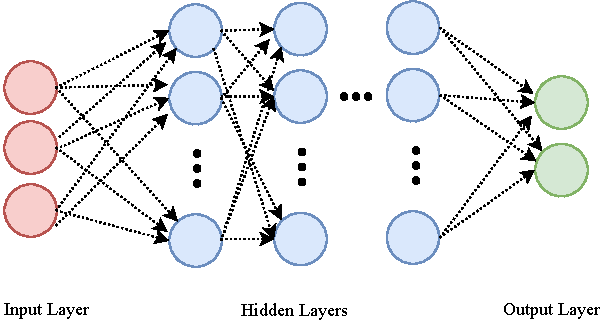
\includegraphics[width=3.0in]{NeuralNetworkFNN.pdf}
% where an .eps filename suffix will be assumed under latex, 
% and a .pdf suffix will be assumed for pdflatex; or what has been declared
% via \DeclareGraphicsExtensions.
\caption{Simple Feed-forward Architecture}
\label{fig_FeedForwardNet}
\end{figure}

\indent Formally, the operation of a neural network can be viewed as a function, $v:I^n \rightarrow O^m$, that maps an $n$-dimensional input, $I^n$, to an $m$-dimensional output, $O^m$ \cite{LeofanteAdvances2018}. For a neural network with $L$ layers, where $1 \leq \ell \leq L$, let $s_\ell$ denote the size of the layer $\ell$, $s_1$ denote the size of the input layer, $v_{\ell,j}$ denote the value of the $j$-th neuron of layer $\ell$, $b_\ell$ be a bias vector of size $s_\ell \times 1$, and $U_\ell=[u_{\ell,1},\dots,u_{\ell,s_\ell}]^T$ be a column vector of neuron activations for layer $\ell$  (\cite{WeimingReachability2018,KatzReluplex2017}). For each layer $2<\ell<L$, there is an associated weight  matrix, $W_\ell$, of size $s_\ell \times s_{\ell-1}$. Thus, the neuron activation vector, $U_\ell$, can be described by:
\begin{equation}
U_\ell=f(W_\ell \cdot U_{\ell-1}+b_l) \label{eq:NN_gen}
\end{equation}
where the activation function $f(\cdot)$ is applied component-wise \cite{KatzReluplex2017}. Given an input, $U_1$, the output of the whole network is given by applying rule (\ref{eq:NN_gen}) repeatedly until $U_\ell$ is calculated. %\cite{KatzReluplex2017}.
\subsection{Convolutional Neural Networks}
Convolutional neural networks (CNN) are very similar to feed-forward networks but make the explicit assumption that the inputs are images \cite{karpathyConv}. Thus, their structure is tailored towards dealing with images in an efficient manner. Since images can be thought of as being organized into three dimensions, namely in terms of height, width, and depth (typically RGB values), CNNs have neurons that are organized with respect to these dimensions. These layers are called \emph{convolutional layers} and consist of a set of learn-able filters that we convolve over the image in order to compute neuron activations. Additionally, in order to limit the number of parameters that must be learned during training, CNNs also include layers called \emph{pooling layers} that perform a down sampling operation on the input volume of the previous layer (\cite{karpathyConv,HuangSafetyVerification2016}). We refer the reader to  the following papers for an in-depth discussion of this class of network (\cite{karpathyConv,HuangSafetyVerification2016}).
\section{Neural Network Verification \label{sec: Verification}}
\subsection{Verification Problem}
The verification problem for neural networks refers to the process of proving that the output of a network satisfies some desirable property for every choice of input within a bounded set \cite{KrishnamurthyDual2018}. To accomplish this, the problem is posed as a search for an input that causes the negation of a desired property to be true. If the search is successful, then we conclude that the property does not hold and the obtained solution serves as a counterexample demonstrating this failure \cite{KatzLecture_2018}. Otherwise, the search fails and we conclude that the property is true.
Formally, the problem can be stated as: given a neural network that maps an input, $x_1$, to an output, $u_1$, via $u_1=v(x_1)$, along with an input domain, $C$, and a property $P$, we wish to prove:
\begin{equation}
    \forall x_1 \in C, \ u_1=v(x_1) \Rightarrow P(u_1)  \label{eq:sat}
\end{equation}
where $P(u_1)$ describes the undesired behavior for the network (\cite{KatzLecture_2018, KrishnamurthyDual2018}). Ultimately, the verification problem is obtained by encoding the network as a constraint system as in (\ref{eq:sat}) and determining whether there exists an assignment that satisfies all of the the constraints \cite{LeofanteAdvances2018}.

The problem posed in (\ref{eq:sat}) is a deeply challenging problem and it has been demonstrated that proving even simple properties about the behavior of neural networks is an NP-complete problem \cite{KatzReluplex2017}. This challenge is primarily caused by the presence of nonlinear activation functions. While, these functions enable neural networks to learn complex mappings, they also make the verification process more difficult \cite{KuperScalableVerification2018}. The principal challenge, as in other realms of verification, is developing techniques that will scale to the size of networks encountered in practice \cite{AlurFormalVerificationHybridSystems}. Currently, the most successful methods deal with feed-forward and convolutional neural networks that make use of piece-wise linear activation functions, such as ReLU and max pooling \cite{BunelPiecewise2017}. The remainder of this section provides an introduction to the procedures commonly used in solving verification problems posed as (\ref{eq:sat}).
\subsection{Satisfiability Modulo Theories} 
Satisfiability Modulo Theories (SMT) generalizes the Boolean satisfiability (SAT) problem, into the problem of finding a series of assignments, called an interpretation, such that a first-order logic formula, with respect to some background theory evaluates to true \cite{LeofanteAdvances2018}. A background theory is a set of sentences in a formal language that can be used to restrict the interpretations considered in the SMT decision problem \cite{BarettSMT}. Commonly considered background theories include: the theory of integers, the theory of real numbers, and the theory of linear arithmetic \cite{KuperScalableVerification2018}. To determine the satisfiability of a given SMT problem, SMT solvers typically build a boolean abstraction of the formula by replacing each constraint in the formula with a boolean variable and use a state-of-the-art SAT solver to search for a satisfying assignment \cite{LeofanteAdvances2018}. If the solver fails to find a satisfying assignment, then the solver concludes that the SMT formula is unsatisfiable. However, if the SAT solver finds a suitable interpretation, a theory solver is used to determine whether or not the interpretation is consistent within the context of the background theory \cite{BarettSMT}. If the solution is inconsistent, the theory solver provides an explanation of the inconsistency and refines the boolean abstraction of the SMT formula \cite{LeofanteAdvances2018}. This process occurs continuously and terminates either when a theory-consistent interpretation has been found or when the boolean abstraction of the formula is found to be unsatisfiable \cite{LeofanteAdvances2018}. 

There are a number of powerful and efficient off-the-shelf SMT solvers \cite{BarettSMT} that are well-suited to the verification of neural networks with piecewise linear activation functions. By encoding properties as in (\ref{eq:sat}), using SMT formulas, researchers have been able to verify feed-forward neural networks with about 1800 neurons \cite{KatzReluplex2017}, and convolutional neural networks with up to 1.25 million learnable parameters \cite{HuangSafetyVerification2016}. %However, SMT methods have not been been able to scale to problems larger than those considered in the aformentioned works.
\vspace{-0.2 cm}
\subsection{Linear and Mixed Integer Programming}
Neural network verification can also be posed as an optimization problem using \emph{Linear} (LP) and \emph{Mixed Integer Programming} (MIP). Mixed Integer Programming is an extension of Linear Programming that involves the optimization of a function over a set of integer and real-valued variables subject to a set of linear constraints \cite{LeofanteAdvances2018}. Traditionally, the problem is described by variables known as \emph{decision variables}, and a linear objective function that we wish to minimize or maximize. Formally this can be expressed as:
\begin{align}
    \textrm{min} &\sum_{j=1}^{n}c_ix_i \label{eq:MIP}\\
    \textrm{subject to}& \sum_{j=1}^{n} a_{ji}x_i \geq b_j, \ \ j \in [1,m] \label{eq:MIP2}
\end{align}
where $x_i \in [a_i, b_i] \cap \mathbb{Z}$ are the bounded decision variables, (\ref{eq:MIP}) is the objective function, and (\ref{eq:MIP2}) are the set of linear constraints that need to be upheld (\cite{LeofanteAdvances2018,KatzLecture_2018}).

To formulate the neural network verification problem as an MIP problem the network must employ the use of piece-wise linear activation functions and the property considered must also be expressible as a set of linear set of constraints. An in-depth discussion of the process of encoding neural networks into MIP problems can be found in the following papers (\cite{BunelPiecewise2017, BastaniMeasuring2018, TjengMixedIntegerPogramming}). %Mixed Integer Programming is a well-studied problem and there are numerous efficient MIP solvers and algorithms for obtaining solutions to MIP problems. %Still, MIP optimization is an NP-hard problem and as a result MIP methods have achieved similar levels of scalability as SMT problems.
\subsection{Other Approaches}
While the SMT and MIP formulations of the neural network verification problem are the most commonly used techniques within the research literature, there are several other notable techniques not characterized by the philosophy of (\ref{eq:sat}). These methods include: \emph{test coverage methods}, and \emph{concolic testing}. Test coverage methods, which draw inspiration from software engineering, are white-box testing methodologies aimed at generating exhaustive test cases to gauge the correctness of a neural network's behavior. There have been a number of promising techniques proposed within this realm and a discussion of these results can be found in the following survey \cite{XiangVerification2018}. 
Concolic testing methods are similar to test coverage methods, however, they combine program execution and symbolic methods in order to explore paths that are hard to cover via test coverage techniques\footnote{We refer readers to the following paper for a discussion of concolic testing methods \cite{SunTesting2018}}. These approaches have largely been successful in testing networks for adversarial input robustness, but do not provide comprehensive assurance that a neural network is free from defect \cite{XiangVerification2018}. The remainder of this paper will focus on SMT and MIP based verification.

\section{Perspectives on Neural Network Verification \label{sec: Perspectives}}
This section presents neural network verification from three perspectives: the first perspective presents a survey and classification of the existing verification methods, the second presents an experimental evaluation of two state-of-the-art software tools designed for networks with piece-wise linear activation functions, and the third perspective classifies verification approaches into two main modes of thought: complete verification techniques and incomplete verification techniques.
\subsection{Leofante et al., Invariance, Invertibility, and Equivalence}
In their survey, Francesco Leofante et al. present a comprehensive categorization of neural network verification schemes into three distinct classes, based on the particular type of property being considered for verification. The three properties that the authors consider are: invariance, invertibility, and equivalence \cite{LeofanteAdvances2018}.
\subsubsection{Invariance}
Verification methods that deal with invariance are described by (\ref{eq:sat}), and Leofante et al. note that the majority of neural network verification methods deal with properties of this nature \cite{XiangVerification2018}. As a result, Leofante et al. note that there are two different notions of invariance: global invariance and local invariance. Techniques that cater to local invariance properties are often concerned with searching for adversarial examples and seek to demonstrate the invariance of a classification decision within a small neighbourhood of a single input (\cite{HuangSafetyVerification2016, NarodytskaVerifying2017}). These techniques are often either posed as a MIP optimization problem, or as an SMT problem. 

Global invariance techniques, on the other hand, deal with properties that consider all inputs within a bounded domain, and as a result, these properties are harder to demonstrate. Currently, the most successful methods have been able to verify neural networks with piece-wise linear activation functions on the order of thousands of neurons (\cite{KatzReluplex2017, KatzLecture_2018, BunelPiecewise2017}). Constrastingly, for networks that make use of more general activation functions, the most successful techniques have only been able to deal with networks on the order of tens to hundreds of neurons \cite{PulinaAbstraction2010}. It is also worth noting that the vast majority of invariance verification techniques deal with networks with feed-forward architectures and Leofante et al. cite only one article capable of dealing with convolutional architectures \cite{HuangSafetyVerification2016}. 
\subsubsection{Invertibility}
The second class of methods that Leofante et al. consider are methods that deal with invertibility. Properties relating to invertibility can be posed similarly to falsification problems within the context of formal methods \cite{XiangVerification2018}. Given an output $u_1=v(x_1)$ that satisfies some property $P(u_1)$ the task is to find an input, $x_1$, such that the input is part of a particular bounded input domain $C$ \cite{LeofanteAdvances2018}. In this regime, the central focus is obtaining a specific input counterexample that causes the network to exhibit some undesired behavior described by $P$. At the time of Leofante et al.'s publication, the authors cited only two articles by Rudiger Ehlers et al. \cite{EhlersFormal2018} and Svyatoslav Korneev \cite{KorneevConstrained2018}, that specifically dealt with neural network invertibility. However, since then, there have been several proposed verification approaches such as  (\cite{WickerFeatureGuided2017,DreossiSemantic2018}). We refer readers to the following survey for a comprehensive exploration of the aforementioned techniques \cite{XiangVerification2018}.
\subsubsection{Equivalence}
Lastly, Leofante et al. examine verification methods that deal with network equivalence. Network equivalence properties involve two distinct networks, and aim to find an input such that the outputs of the networks are dissimilar. Properties relating to network equivalence are popular within studies that consider adversarial input robustness, and in this context, researchers wish to guage whether or not an adversarial example discovered for a specific neural network, will also be incorrectly classified by a network that is trained on a separate set of data. Formally, this can be described by:
\begin{align}
    \forall x_1 \in C, \ (u_1=v(x_1) \Rightarrow P(u_1) \ \wedge \\ u_2=v'(x_1) \Rightarrow Q(u_2)) \Rightarrow u1=u_2 \label{eq:sat} \notag  
\end{align}
where $x_1$ is a bounded input, $v(x)$ and $v'(x)$ are the functions implemented by the two networks, and $Q(x)$ and $P(x)$ are properties relating to the the network outputs $u_1$ and $u_2$ \cite{LeofanteAdvances2018}. Although there are several adversarial input robustness studies that consider a local flavor of this problem, Leofante et al. cite only work by Narodystka et al. \cite{NarodytskaVerifying2017} that specifically deals with global formulation of this problem as given by (\ref{eq:sat}). Thus, the authors cite this as a potential area of interest for further investigation.
\subsection{Bunel et al.'s Unified View of Piece-wise Linear Neural Network Verification}
While Leofante et al.'s survey presents a comprehensive categorization of verification methodologies, another survey by Rudy Bunel et al. \cite{BunelPiecewise2017}, provides an experimental evaluation of two efficient verification software tools for piece-wise linear neural networks, on a set of benchmark problems with closely related properties. The authors argue that verification methods that deal with networks with piece-wise linear activation functions can be viewed as special cases of branch and bound optimization. By formulating the verification problem in this fashion, the authors designed a novel software tool that surpassed the performance of state-of-the-art methods at that time.
\subsubsection{Branch and Bound Optimization}
 Bunel et al. assert that verification problems formulated as satisfiability problems, as in (\ref{eq:sat}), can be reduced to a global optimization problem where the satisfiability of a formula will be obtained by checking the sign of the minimum. Thus, given a property $P(u_1)$ that can be expressed as boolean formula over linear inequalities, the authors add an additional layer to the network with one output that represents the property considered for verification \cite{BunelPiecewise2017}. As an example, Bunel et al. state, that for a property expressed as linear inequality given by $P(u_1)=c\cdot u_1 \geq b$, one can add a final layer with connection weights given by the vector, $c$, and a bias vector given by $-b$ \cite{BunelPiecewise2017}. With the addition of this layer, the verification problem is reduced to finding an input such that the output of the network is negative. If the output is negative, then the value given by an MIP optimizer is a counterexample. Otherwise, if the output is positive, then we can conclude that the property is satisfied. The authors assert that the advantage of formulating the problem in this fashion, is that one can construct and prove several complex properties at once without having to create and run multiple instances of (\ref{eq:sat}) as in other approaches (\cite{KatzReluplex2017, EhlersFormal2018}). An in-depth discussion of these techniques as well as the reduction of piece-wise linear verification procedures to branch and bound optimization can be found in \cite{BunelPiecewise2017}.
\subsubsection{Reluplex and Planet}
The two verification tools that Bunel et al. consider for experimental evaluation are Reluplex,\footnote{Guy Katz et al.'s verification tool Reluplex is available at \url{https://github.com/guykatzz/ReluplexCav2017}} designed by Guy Katz et al. \cite{KatzReluplex2017}, and Planet,\footnote{R\"{u}diger Ehlers et al.'s verification tool Planet is available at \url{https://github.com/progirep/planet}} developed by R\"{u}diger Ehlers et al. \cite{EhlersFormal2018}. Reluplex is a specialized SMT solver for verifying neural networks that make use of ReLU activation functions. The tool is based on an extension of the simplex algorithm \cite{Nelder1965} in linear optimization, that allows the authors to efficiently deal with SMT formulas that encode ReLU constraints. During the search for a satisifiable assignment to a query such as in (\ref{eq:sat}), the principle of Reluplex is to always maintain an assignment to all of the variables even if some of the ReLU constraints are violated \cite{KatzReluplex2017}. As the search progresses, at each step, Reluplex tries to fix a violated constraint and terminates either when a satisfying example is obtained or if the search fails to find a solution. In their paper, the authors demonstrate that Reluplex can handle networks with up to 1800 neurons (\cite{KatzReluplex2017}\cite{LeofanteAdvances2018}).

Correspondingly, Ehlers et al.'s tool, Planet, is based on an approach that leverages both SMT and MIP solvers \cite{EhlersFormal2018}. In their framework, the authors make use of a linear approximation of the neural network's behavior, in order to prune the search space that the solvers must consider during execution. Given a particular linear constraint system encoding of a network, Planet tries to find a satisfying interpretation, and at each step, the tool assigns a value of 0 or 1 to each variable associated with ReLU ($\textrm{max}(0,x)$) or pooling functions. If a satisfying solution is found, the tool returns the solution as counterexample. Otherwise, if there are no solutions corresponding to the current partial assignment, the tool backtracks, and attempts a different assignment. This search is done iteratively until either a satisfying solution is found, or if the solver concludes that no solution exists (\cite{EhlersFormal2018, KatzLecture_2018}). In their work, Ehlers et al. demonstrate that they are able to prove properties for networks with over 1341 neurons.
\subsubsection{Experimental Results}
To assess the performance of the aformentioned tools, Bunel et al. utilized three benchmark data sets with a diverse set of properties considered for verification and of varying dimensionality \cite{BunelPiecewise2017}. The results of their experiments, demonstrated that by expressing neural network verification as a branch and bound optimization problem, their software tool was able to surpass the performance of Reluplex and Planet \cite{BunelPiecewise2017}. In some cases, their tool executed with a speedup of over two orders of magnitude. However, despite significant improvements in run-time, the authors did not present an evaluation of whether their tool achieved better scalability than the methods proposed by Katz et al. and Ehlers et al. Thus, it is unclear whether or not Bunel et al.'s methods are superior to those of Reluplex and Planet. This is an interesting question that merits further investigation\footnote{A detailed summary of the experimental results of Bunel's experiments can be found online at \url{https://github.com/oval-group/PLNN-verification}, and in the following paper \cite{BunelPiecewise2017}}.
\begin{table*}
	\scalebox{0.9}{{}\begin{tabular}{  c | c | c  | c | c | c} 
		Tool Name & Network Type & Verification Approach & Largest Network Considered & Completeness & Type of Property\\
		\hline
		\href{https://github.com/guykatzz/ReluplexCav2017}{Reluplex} \cite{KatzReluplex2017} & FNN & SMT & 1800 neurons & Complete & Invariance \\
		\href{https://github.com/progirep/planet}{Planet}  \cite{EhlersFormal2018} & FNN, CNN & SMT, MIP & 1341 neurons & Complete & Invariance, Invertibility \\
		\href{https://github.com/oval-group/PLNN-verification}{PLNN} \cite{BunelPiecewise2017} & FNN, CNN & Branch and Bound & 1485 & Complete & Invariance\\
        \href{https://github.com/souradeep-111/sherlock}{Sherlock} \cite{DuttaOutputRange2017} & FNN & MIP & 3822 & Complete & Invariance \\
        \href{https://github.com/VeriDeep/DLV}{VeriDeep/DLV}\cite{HuangSafetyVerification2016}  & FNN, CNN & SMT & $1.25 \times 10^6$  parameters & Incomplete & Invariance \\
        \href{https://github.com/Microsoft/NeuralNetworkAnalysis}{NNAF} \cite{BastaniMeasuring2018} & CNN & LP & 60000 parameters & Incomplete & Invariance \\
        \href{https://github.com/Microsoft/NeuralNetworkAnalysis}{MIPVerify.jl} \cite{TjengMixedIntegerPogramming} & FNN, CNN & MIP & 500 neurons & Incomplete & Invariance, Invertibility \\
        \href{http://ai2.ethz.ch/}{$\textrm{AI}^2$} \cite{GehrAI} & FNN, CNN & Abstract Interpretation & 53000 neurons & Incomplete & Invariance\\
        \hline
    \end{tabular}}
    \caption {Summary of several available software tools for network verification present in the research literature. A more comprehensive list of tools can be found in \cite{XiangVerification2018}.}\label{tab:tools}
\end{table*}

\subsection{Modes of thought within Neural Network Verification}
The last perspective we consider in this paper is a categorization of neural network verification methods into two main modes of thought, as described by Guy Katz in \cite{KatzReluplex2017}. One of the greatest challenges in verification is designing methods that scale well to real world applications. To address this challenge, two types of techniques have arisen in the research literature: methods that are sound and complete, and methods that are sound and incomplete. \cite{KatzLecture_2018}. Intuitively, a sound method is a method that always returns a correct answer, and a complete method is one that is guaranteed to find a solution if one exists \cite{KatzLecture_2018}. Katz asserts that techniques which are sound and complete are typically limited in terms of scalability. As a result  these methods have been able to deal with networks with sizes on the order of hundreds to thousands of neurons. As an example, Reluplex and Planet are techniques that are both sound and complete, and there are a number of other approaches that fall within this category (\cite{TjengMixedIntegerPogramming,XiangVerification2018,DuttaOutputRange2017,LomuscioReachability2017}). A summary of the existing software tools can be found in Table \ref{tab:tools}.

On the other hand, sound and incomplete techniques exhibit better scalability and can handle networks with thousands to tens of thousands of neurons \cite{KatzReluplex2017}. While these techniques are superior in terms of scalability, they may not return an answer to the specific verification problem posed by the researcher. However, these approaches often work well in practice and there have been a number of notable approaches proposed in recent years. A discussion of these methods can be found in \cite{HuangSafetyVerification2016} and \cite{ XiangVerification2018}. For instance, in their paper, Osbert Bastani et al. present a method for deriving adversarial inputs with some neighborhood of an input image \cite{BastaniMeasuring2018}. While their methods can generate adversarial examples, if they exist, they cannot guarantee that there are no other adversarial examples within this region to be discovered. Katz notes that comparing complete and incomplete techniques is difficult, and in the future, an analysis of the benefits and drawbacks of both methods merits investigation.
\section{Major Challenges and Future Work \label{sec: Challenges}}
The last several years have witnessed a significant increase in the the number of proposed verification methods for neural networks \cite{XiangVerification2018}. Currently the vast majority of research efforts have focused on designing methods that scale to networks utilized in real world applications. Unfortunately, networks such as GoogLeNet, AlexNet, and VGGNet that contain millions of neurons (\cite{BallesterGoogLeNet,SimonyanVeryDeep}) are currently out of reach. The current limiting factor in these efforts is an effective treatment of the non-linearities introduced by activation functions, and at the present time, the vast majority of methods can only handle functions that are piecewise linear \cite{KuperScalableVerification2018}. Regrettably, it is not clear how this problem can be overcome, and thus there is an urgent need for the additional research towards the development of methods that will work well in practice. 

In addition to creating more scalable methods, there are several other open problems within this realm. Presently, there is a lack of effective methodology for comparing the existing verification techniques due to the diversity of the underlying SMT and SAT solvers utilized in state-of-the-art tools, a lack of standardized benchmarks, distinct verification modes of thought, and a great variety of properties considered for verification. In fact, Guy Katz notes that often the property being considered for verification has a large influence on the complexity of the problem \cite{KatzReluplex2017}. Moreover, there is a lack of a standardized input format describing neural network verification problems for the available software tools within the community. As a result, it is difficult for researchers to efficiently and accurately evaluate the success of their techniques.

Lastly, while the vast majority of the existing verification methods can provide examples that are realizations of undesired behavior, they have not yet provided an intuitive way of creating models that are free from defect. Due to the opaqueness of neural network models, techniques that describe how to modify a network's structure to cause the network to satisfy some desirable property would be extremely useful \cite{KatzReluplex2017}.

In light of these challenges, there are several interesting directions for future work including:
\begin{itemize}
    \item The creation of standardized benchmark sets and input formats for the effective evaluation of proposed verification methods,
    \item Constructing SMT and SAT solvers that are specifically designed to handle formulas that involve neural network constraints such as Reluplex (\cite{KatzReluplex2017, KuperScalableVerification2018}),
    \item A comprehensive cost-benefit analysis of complete and incomplete neural network verification approaches,
    \item Interdisciplinary studies towards the creation of interpretable neural network models from domain experts from the Artificial Intelligence and Automated Verification communities
    \item And further research into other forms of verification such as run-time monitoring for systems that incorporate neural networks into their architecture. 
\end{itemize}
If the research community can obtain acceptable solutions to the aforementioned challenges, they will stimulate the development of robust and intelligent systems with the potential to bring unparalleled benefits to numerous application domains. Moreover, they will provide the basis for theoretical and practical advances within artificial intelligence and automated verification.




%\section{Conclusion}





% if have a single appendix:
%\appendix[Proof of the Zonklar Equations]
% or
%\appendix  % for no appendix heading
% do not use \section anymore after \appendix, only \section*
% is possibly needed

% use appendices with more than one appendix
% then use \section to start each appendix
% you must declare a \section before using any
% \subsection or using \label (\appendices by itself
% starts a section numbered zero.)
%


%\appendices
%\section{Proof of the First Zonklar Equation}
%\blindtext

% use section* for acknowledgement
%\section*{Acknowledgment}


%The authors would like to thank...


% Can use something like this to put references on a page
% by themselves when using endfloat and the captionsoff option.
\ifCLASSOPTIONcaptionsoff
  \newpage
\fi



% trigger a \newpage just before the given reference
% number - used to balance the columns on the last page
% adjust value as needed - may need to be readjusted if
% the document is modified later
%\IEEEtriggeratref{8}
% The "triggered" command can be changed if desired:
%\IEEEtriggercmd{\enlargethispage{-5in}}

% references section

% can use a bibliography generated by BibTeX as a .bbl file
% BibTeX documentation can be easily obtained at:
% http://www.ctan.org/tex-archive/biblio/bibtex/contrib/doc/
% The IEEEtran BibTeX style support page is at:
% http://www.michaelshell.org/tex/ieeetran/bibtex/
%\bibliographystyle{IEEEtran}
% argument is your BibTeX string definitions and bibliography database(s)
%\bibliography{IEEEabrv,../bib/paper}
%
% <OR> manually copy in the resultant .bbl file
% set second argument of \begin to the number of references
% (used to reserve space for the reference number labels box)

% biography section
% 
% If you have an EPS/PDF photo (graphicx package needed) extra braces are
% needed around the contents of the optional argument to biography to prevent
% the LaTeX parser from getting confused when it sees the complicated
% \includegraphics command within an optional argument. (You could create
% your own custom macro containing the \includegraphics command to make things
% simpler here.)
%\begin{biography}[{\includegraphics[width=1in,height=1.25in,clip,keepaspectratio]{mshell}}]{Michael Shell}
% or if you just want to reserve a space for a photo:
\bibliographystyle{IEEEtran}
\bibliography{prelim.bib}
\end{document}
%\begin{IEEEbiography}[{\includegraphics[width=1in,height=1.25in,clip,keepaspectratio]{picture}}]{John Doe}
%\blindtext
%\end{IEEEbiography}

% You can push biographies down or up by placing
% a \vfill before or after them. The appropriate
% use of \vfill depends on what kind of text is
% on the last page and whether or not the columns
% are being equalized.

%\vfill

% Can be used to pull up biographies so that the bottom of the last one
% is flush with the other column.
%\enlargethispage{-5in}




% that's all folks



